\qitem{%
    Let $ABC$ be an acute triangle with $AB >AC$ and $\angle BAC =60^o$. Denote the circumcenter by $O$ and orthocenter by $H$. The extension of $OH$ intersects $AB$ and $AC$ in $P$ and $Q$ respectively. Prove that $PO=HQ$.
    }{%
    $AH = 2R\cos 60^\circ = R = AO, \angle PAO=\angle QAH=90^\circ-\angle C, \angle AOP=\angle AHQ.$ Thus, triangles $APO, AQH$ are congruent and $PO=QH$.

    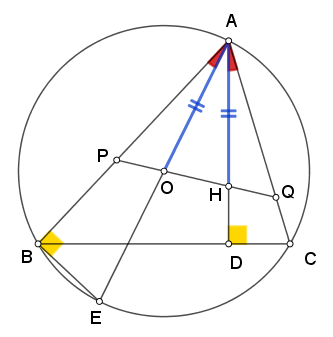
\includegraphics[width=0.3\linewidth]{./go5_pic/go5_ans_POequalHQ.png}
    }{%
    https://artofproblemsolving.com/community/c4t70430f4h1849571_equal_segments_orthocenter_and_circumcenter_related
}

